\chapter{Implementation Overview}
As already said the aim of the project is to provide a secure PUF to recognize IoT devices, in order to avoid impersonation attacks.

The type of PUF implemented is a SRAM PUF (parlare un attimo dell' SRAM PUF se non e' stato fatto prima), this was implemented using a SECube device.

The Idea is that the first time an Host is connected to the SECube, it asks the device all the PUFs that it has collected during its starting phases.
This challenge and response information has to be stored by the host in a cipher way:
\begin{equation}\label{eq:eq1}
 data\_to\_store=H(response)
 \end{equation}
 
  the challenge has to stay in plaintext.

In the future when the host has to establish a connection with the device, he is going to send to it a specific challenge, the device is going to answer with a response;
then the host has to check the validity of the response, evaluating the digest and comparing with the one that he has in the storage file.
Once a challenge-response is used, it has to be eliminated and not used anymore in the future; in this way it is possible to avoid replicant attacks.


The implementation of this project can be divided in two flow:
\begin{enumerate}
	\item The first flow consists in the exchange of all the challenge and response information between host and device 
	\item The second flow consists in the challenge and response authentication of the device
\end{enumerate}

Here will be explained only a general idea of the implementation and in the next chapter will be described deeply the functioning.

\begin{figure}[H]
\centering
  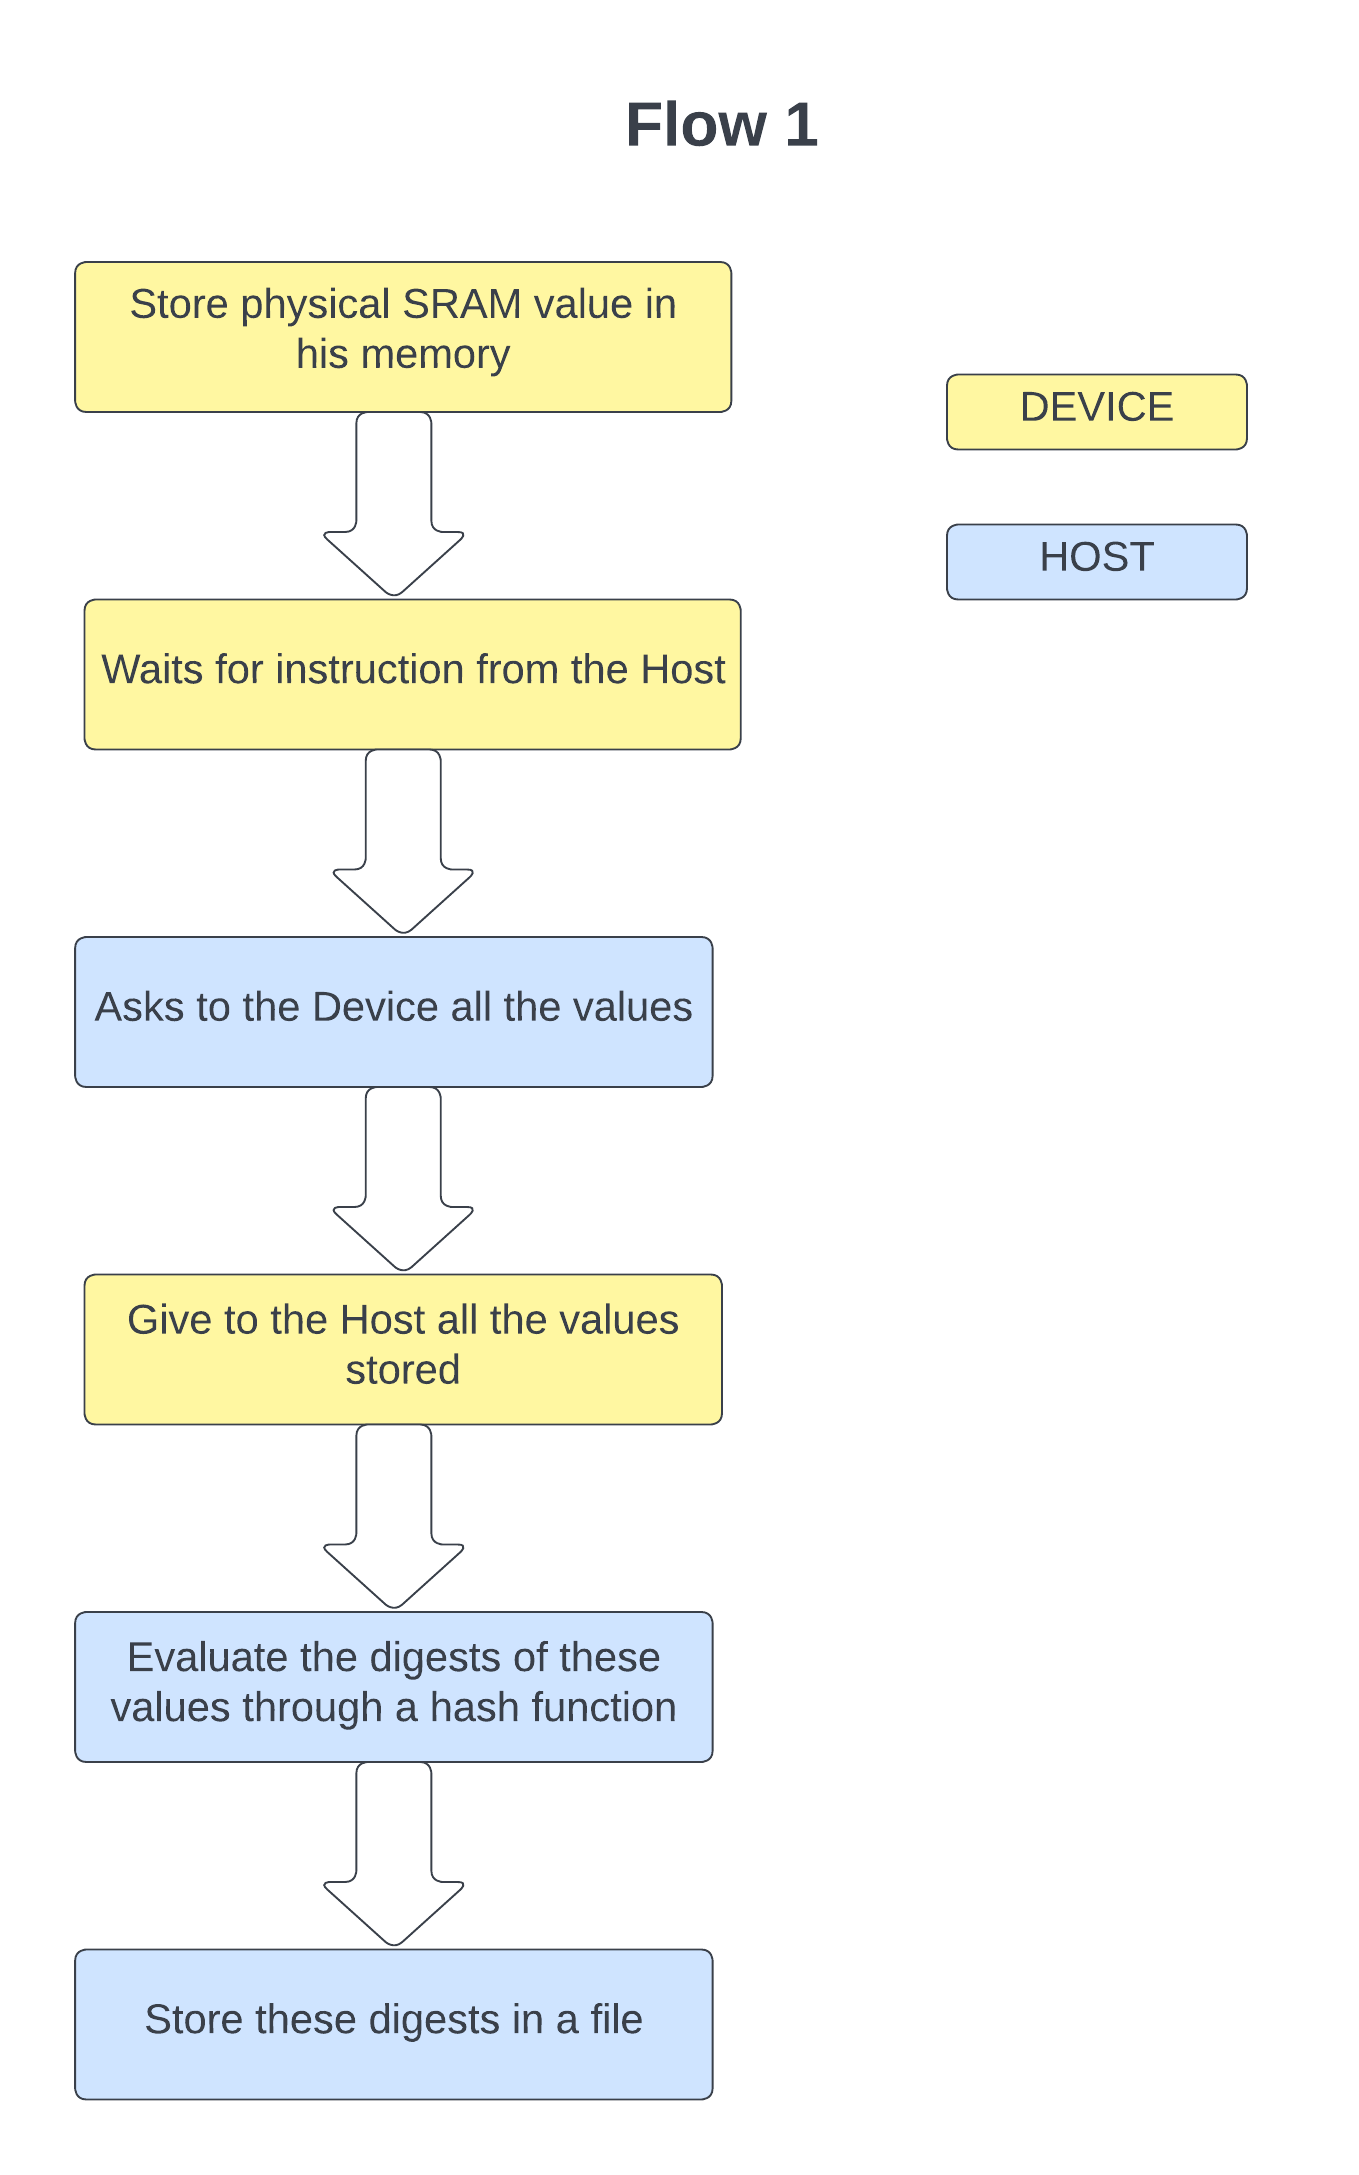
\includegraphics[width=5cm]{images/flow_1.png}
  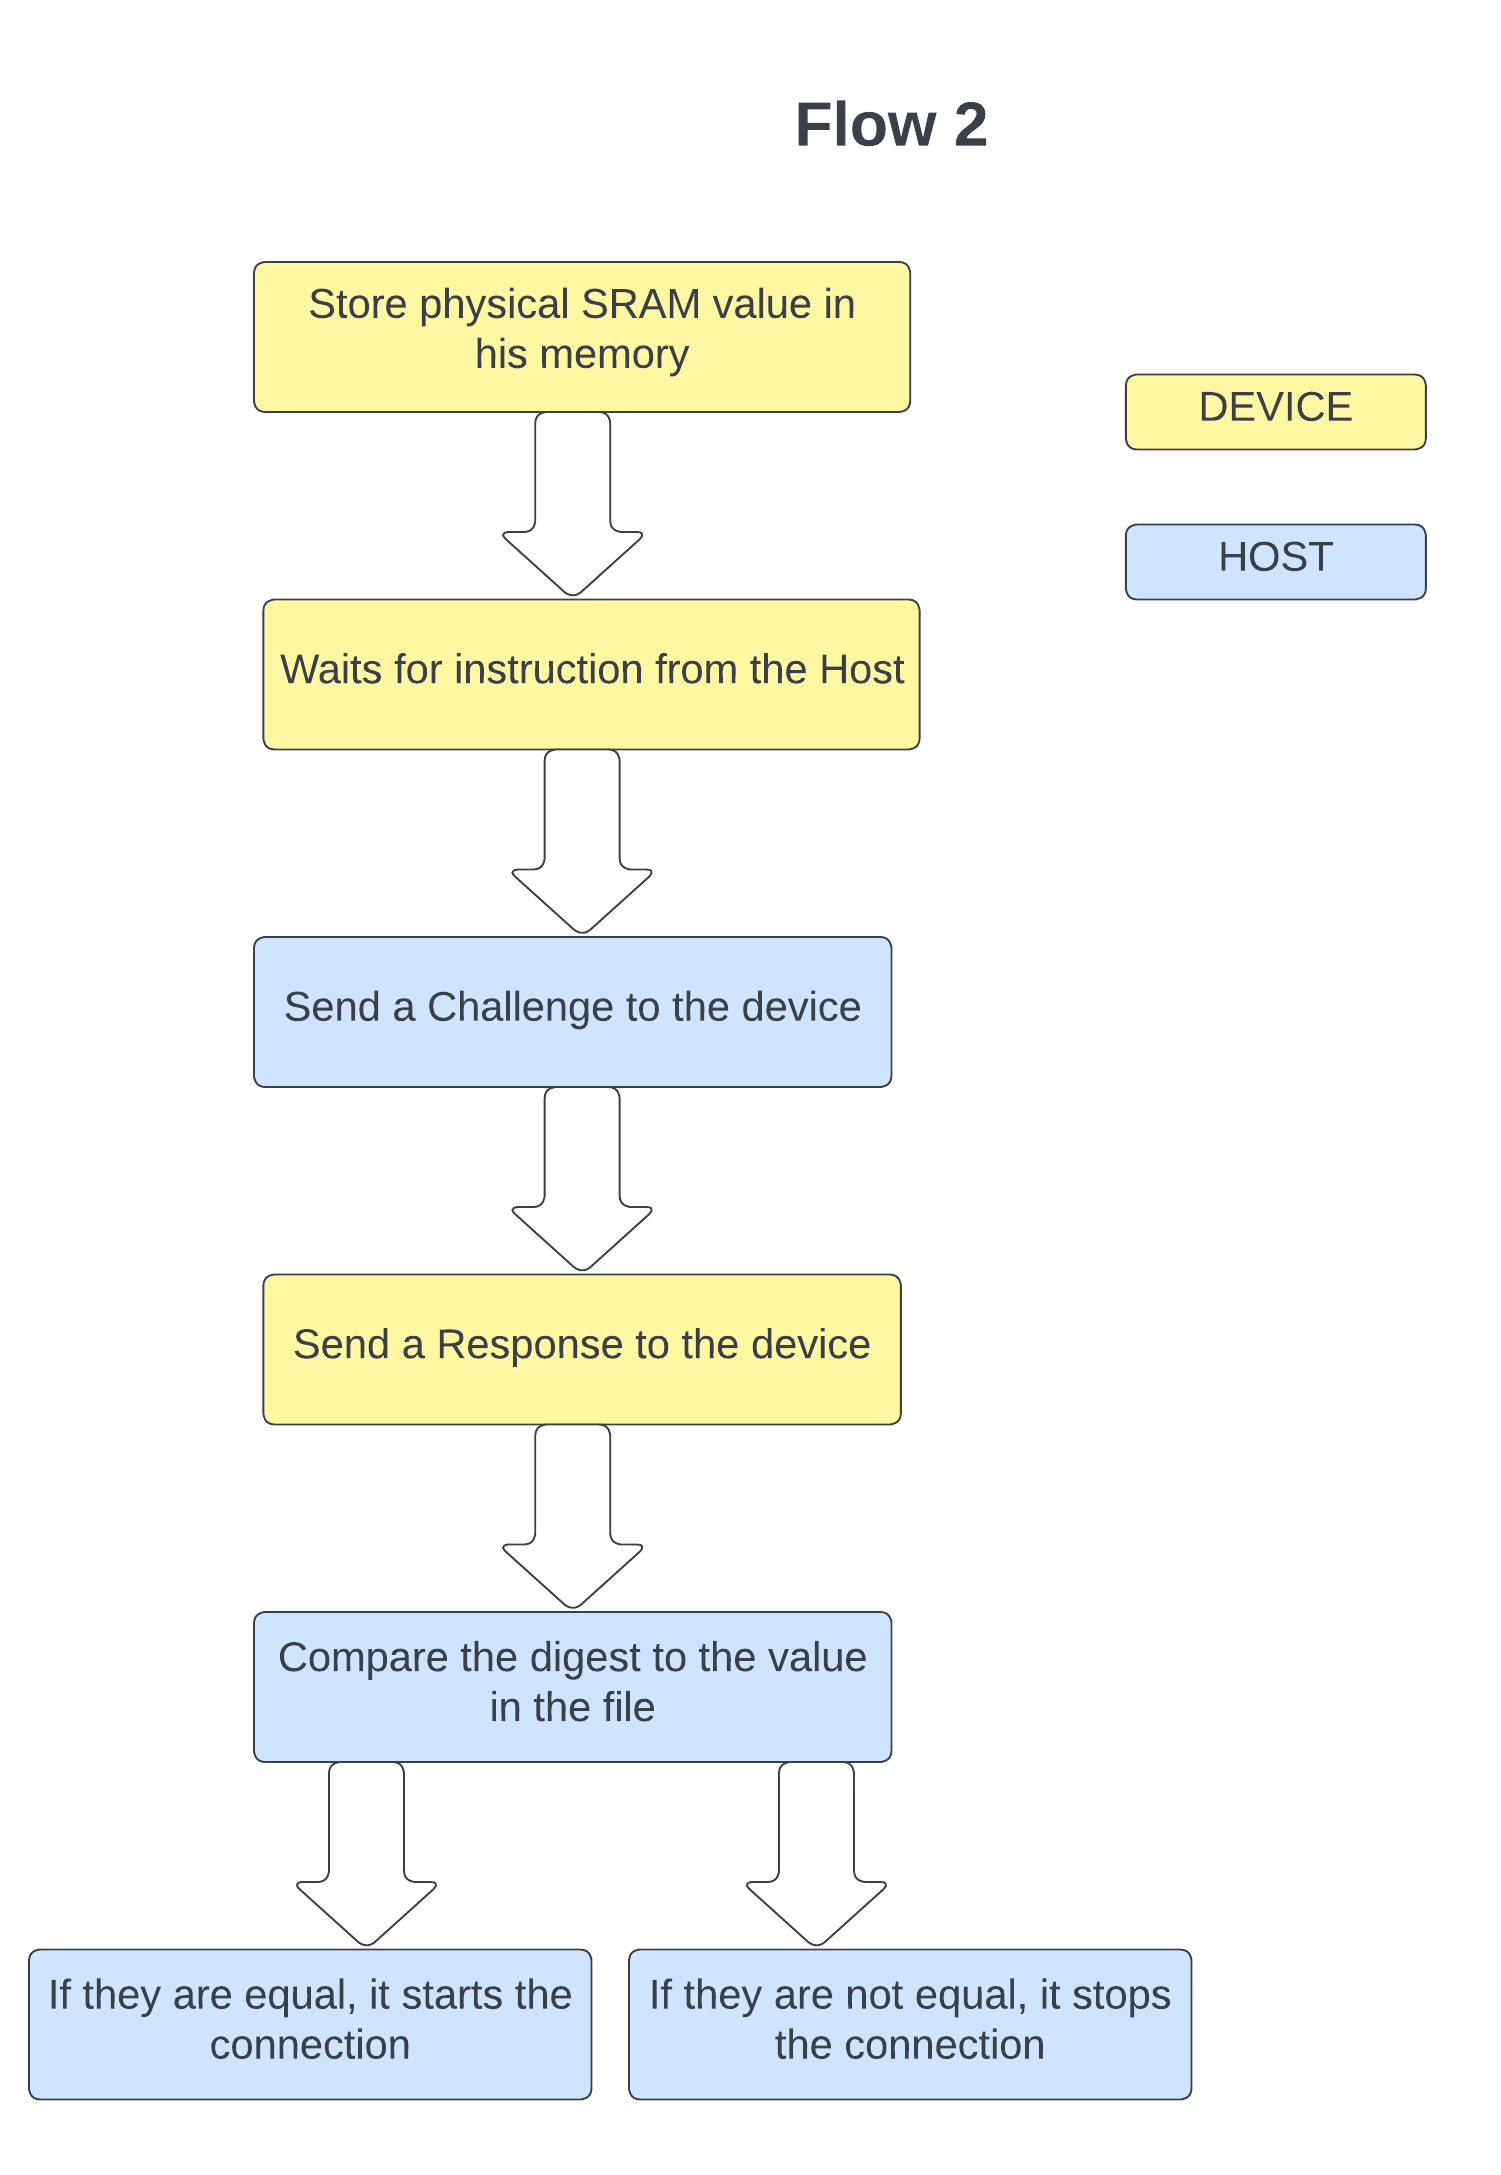
\includegraphics[width=5cm]{images/flow_2.png}
  \caption{Flow 1 and Flow 2}
  \label{fig:sub2}
\end{figure}

\section {Device side} 
On the device side both of the flows have a common important operation that has to be done. This operation consists in taking the values present in the SRAM when this one is switched on and storing them in a secure place. Obviously this operation is the first operation that has always been done by the device as soon as it is switched on.

Secondly, if this is the first time that it communicates with this particular host it waits until the host asks it for all the value that it has just taken from the SRAM in order to implement the challenge-response authentication for the next time.

On the other hand, it waits until the host sends to it a particular challenge, this challenge will be the index of a determined response, so the device takes the response and sends them to the host.
After that the device is authenticated and the can starts to communicate.



\section {Host side} 
On the host side the type of work is a little bit different from the device side.
When the connection is instantiated with the device for the first time it asks the device all the values needed to implement the challenge-response authentication; the Host is going to store the hash values of these datas in a file.

During all the next connections with the device, the Host sends a particular challenge to the device and waits for the respective response.
After it receives it, It is going to evaluate the digest of this value, it gives it in input to the hash function and it compares it with the value that it has inside the file.

If the two digests are the same it means that the device is the correct one and so the connection can start; otherwise the host stops the connection.



%In this chapter you should provide a general overview of the project, explaining what you have implemented staying at a high-level of abstraction, without going too much into the details. Leave details for the implementation chapter. This chapter can be organized in sections, such as goal of the project, issues to be solved, solution overview, etc.\\It is very important to add images, schemes, graphs to explain the original problem and your solution. Pictures are extremely useful to understand complex ideas that might need an entire page to be explained.\\Use multiple sections to explain the starting point of your project, the last section is going to be the high-level view of your solution...so take the reader in a short `journey` to showcase your work.
